% Options for packages loaded elsewhere
\PassOptionsToPackage{unicode}{hyperref}
\PassOptionsToPackage{hyphens}{url}
%
\documentclass[
]{article}
\usepackage{amsmath,amssymb}
\usepackage{lmodern}
\usepackage{iftex}
\ifPDFTeX
  \usepackage[T1]{fontenc}
  \usepackage[utf8]{inputenc}
  \usepackage{textcomp} % provide euro and other symbols
\else % if luatex or xetex
  \usepackage{unicode-math}
  \defaultfontfeatures{Scale=MatchLowercase}
  \defaultfontfeatures[\rmfamily]{Ligatures=TeX,Scale=1}
\fi
% Use upquote if available, for straight quotes in verbatim environments
\IfFileExists{upquote.sty}{\usepackage{upquote}}{}
\IfFileExists{microtype.sty}{% use microtype if available
  \usepackage[]{microtype}
  \UseMicrotypeSet[protrusion]{basicmath} % disable protrusion for tt fonts
}{}
\makeatletter
\@ifundefined{KOMAClassName}{% if non-KOMA class
  \IfFileExists{parskip.sty}{%
    \usepackage{parskip}
  }{% else
    \setlength{\parindent}{0pt}
    \setlength{\parskip}{6pt plus 2pt minus 1pt}}
}{% if KOMA class
  \KOMAoptions{parskip=half}}
\makeatother
\usepackage{xcolor}
\usepackage[margin=1in]{geometry}
\usepackage{color}
\usepackage{fancyvrb}
\newcommand{\VerbBar}{|}
\newcommand{\VERB}{\Verb[commandchars=\\\{\}]}
\DefineVerbatimEnvironment{Highlighting}{Verbatim}{commandchars=\\\{\}}
% Add ',fontsize=\small' for more characters per line
\usepackage{framed}
\definecolor{shadecolor}{RGB}{248,248,248}
\newenvironment{Shaded}{\begin{snugshade}}{\end{snugshade}}
\newcommand{\AlertTok}[1]{\textcolor[rgb]{0.94,0.16,0.16}{#1}}
\newcommand{\AnnotationTok}[1]{\textcolor[rgb]{0.56,0.35,0.01}{\textbf{\textit{#1}}}}
\newcommand{\AttributeTok}[1]{\textcolor[rgb]{0.77,0.63,0.00}{#1}}
\newcommand{\BaseNTok}[1]{\textcolor[rgb]{0.00,0.00,0.81}{#1}}
\newcommand{\BuiltInTok}[1]{#1}
\newcommand{\CharTok}[1]{\textcolor[rgb]{0.31,0.60,0.02}{#1}}
\newcommand{\CommentTok}[1]{\textcolor[rgb]{0.56,0.35,0.01}{\textit{#1}}}
\newcommand{\CommentVarTok}[1]{\textcolor[rgb]{0.56,0.35,0.01}{\textbf{\textit{#1}}}}
\newcommand{\ConstantTok}[1]{\textcolor[rgb]{0.00,0.00,0.00}{#1}}
\newcommand{\ControlFlowTok}[1]{\textcolor[rgb]{0.13,0.29,0.53}{\textbf{#1}}}
\newcommand{\DataTypeTok}[1]{\textcolor[rgb]{0.13,0.29,0.53}{#1}}
\newcommand{\DecValTok}[1]{\textcolor[rgb]{0.00,0.00,0.81}{#1}}
\newcommand{\DocumentationTok}[1]{\textcolor[rgb]{0.56,0.35,0.01}{\textbf{\textit{#1}}}}
\newcommand{\ErrorTok}[1]{\textcolor[rgb]{0.64,0.00,0.00}{\textbf{#1}}}
\newcommand{\ExtensionTok}[1]{#1}
\newcommand{\FloatTok}[1]{\textcolor[rgb]{0.00,0.00,0.81}{#1}}
\newcommand{\FunctionTok}[1]{\textcolor[rgb]{0.00,0.00,0.00}{#1}}
\newcommand{\ImportTok}[1]{#1}
\newcommand{\InformationTok}[1]{\textcolor[rgb]{0.56,0.35,0.01}{\textbf{\textit{#1}}}}
\newcommand{\KeywordTok}[1]{\textcolor[rgb]{0.13,0.29,0.53}{\textbf{#1}}}
\newcommand{\NormalTok}[1]{#1}
\newcommand{\OperatorTok}[1]{\textcolor[rgb]{0.81,0.36,0.00}{\textbf{#1}}}
\newcommand{\OtherTok}[1]{\textcolor[rgb]{0.56,0.35,0.01}{#1}}
\newcommand{\PreprocessorTok}[1]{\textcolor[rgb]{0.56,0.35,0.01}{\textit{#1}}}
\newcommand{\RegionMarkerTok}[1]{#1}
\newcommand{\SpecialCharTok}[1]{\textcolor[rgb]{0.00,0.00,0.00}{#1}}
\newcommand{\SpecialStringTok}[1]{\textcolor[rgb]{0.31,0.60,0.02}{#1}}
\newcommand{\StringTok}[1]{\textcolor[rgb]{0.31,0.60,0.02}{#1}}
\newcommand{\VariableTok}[1]{\textcolor[rgb]{0.00,0.00,0.00}{#1}}
\newcommand{\VerbatimStringTok}[1]{\textcolor[rgb]{0.31,0.60,0.02}{#1}}
\newcommand{\WarningTok}[1]{\textcolor[rgb]{0.56,0.35,0.01}{\textbf{\textit{#1}}}}
\usepackage{graphicx}
\makeatletter
\def\maxwidth{\ifdim\Gin@nat@width>\linewidth\linewidth\else\Gin@nat@width\fi}
\def\maxheight{\ifdim\Gin@nat@height>\textheight\textheight\else\Gin@nat@height\fi}
\makeatother
% Scale images if necessary, so that they will not overflow the page
% margins by default, and it is still possible to overwrite the defaults
% using explicit options in \includegraphics[width, height, ...]{}
\setkeys{Gin}{width=\maxwidth,height=\maxheight,keepaspectratio}
% Set default figure placement to htbp
\makeatletter
\def\fps@figure{htbp}
\makeatother
\setlength{\emergencystretch}{3em} % prevent overfull lines
\providecommand{\tightlist}{%
  \setlength{\itemsep}{0pt}\setlength{\parskip}{0pt}}
\setcounter{secnumdepth}{-\maxdimen} % remove section numbering
\ifLuaTeX
  \usepackage{selnolig}  % disable illegal ligatures
\fi
\IfFileExists{bookmark.sty}{\usepackage{bookmark}}{\usepackage{hyperref}}
\IfFileExists{xurl.sty}{\usepackage{xurl}}{} % add URL line breaks if available
\urlstyle{same} % disable monospaced font for URLs
\hypersetup{
  pdftitle={Tourism demand and revenue with sptial effects},
  hidelinks,
  pdfcreator={LaTeX via pandoc}}

\title{Tourism demand and revenue with sptial effects}
\author{}
\date{\vspace{-2.5em}2023-03-20}

\begin{document}
\maketitle

\hypertarget{requirements}{%
\subsection{Requirements}\label{requirements}}

\hypertarget{external-libraries}{%
\subsubsection{External libraries}\label{external-libraries}}

For Linux and macOS (I'm in M2) users who are working with spatial data
in R, you may encounter error messages like this during package
downloading (if you run \texttt{install.packages("sf")}, for example).

\begin{verbatim}
*configure: error: libproj or sqlite3 not found in standard or given locations.*
\end{verbatim}

This is because they need additional (non-R) libraries such as PROJ,
GDAL or GEOS (which are automatically installed for Windows users). It
is highly recommend to install the CRAN binary packages by running in R
terminal

\begin{Shaded}
\begin{Highlighting}[]
\FunctionTok{install.packages}\NormalTok{(}\StringTok{"sf"}\NormalTok{, }\AttributeTok{type =} \StringTok{"mac.binary"}\NormalTok{)}
\end{Highlighting}
\end{Shaded}

If you do want to download the source package, you should refer to
\url{https://r-spatial.github.io/sf/\#macos} and and use the similiar
specification like \texttt{configure.args\ =} for additional
configuration.

\hypertarget{r-packages}{%
\subsubsection{R packages}\label{r-packages}}

Load and install the R packages we might will be using.(This is an
inclusive list, and I did this purposely for future reference. Comment
those not useful in the codes.) See here

\begin{Shaded}
\begin{Highlighting}[]
\DocumentationTok{\#\# Download(if needed) and load package management tool.}
\ControlFlowTok{if}\NormalTok{ (}\SpecialCharTok{!}\FunctionTok{require}\NormalTok{(}\StringTok{"pacman"}\NormalTok{)) }\FunctionTok{install.packages}\NormalTok{(}\StringTok{"pacman"}\NormalTok{)}
\DocumentationTok{\#\# Download(if needed) and load other package for spatial analysis.}
\DocumentationTok{\#\# pacman::p\_load(sf, tidyverse, data.table, hrbrthemes, lwgeom, rnaturalearth, maps, mapdata, spData, tigris, tidycensus, leaflet, mapview, tmap, tmaptools, zoo, pspatreg, spatialreg, spdep, sf, plm, splm, pspatreg)}
\DocumentationTok{\#\# Download(if needed) and load other package for use in this document.}
\NormalTok{pacman}\SpecialCharTok{::}\FunctionTok{p\_load}\NormalTok{(sf, tidyverse, data.table, hrbrthemes, pspatreg, spatialreg, spdep, sf, plm, splm, pspatreg, zoo)}
\DocumentationTok{\#\# ggplot2 plotting theme}
\CommentTok{\# theme\_set(hrbrthemes::theme\_ipsum())}
\end{Highlighting}
\end{Shaded}

\begin{Shaded}
\begin{Highlighting}[]
\DocumentationTok{\#\# Download and load our companion package.}
\DocumentationTok{\#\# devtools::install\_github("JLCHEN0115/spatial2023")}
\DocumentationTok{\#\# library("spatial2023")}
\end{Highlighting}
\end{Shaded}

\hypertarget{data-wrangling}{%
\subsection{Data wrangling}\label{data-wrangling}}

\hypertarget{reading-in-the-spatial-data.}{%
\subsubsection{Reading in the spatial
data.}\label{reading-in-the-spatial-data.}}

Here I will use the absolute path. Replace the path of the
\texttt{cities\_included.shp} file on your computer. The data will be
included in the companion package later on.

\begin{Shaded}
\begin{Highlighting}[]
\CommentTok{\# Replace the absolute path of the \textasciigrave{}cities\_included.shp\textasciigrave{} file on your computer. }
\CommentTok{\# Drag the file to terminal (command + space, then search \textasciigrave{}terminal\textasciigrave{} on spotlight) if you are in mac, the path will appear.}
\NormalTok{ct\_shape }\OtherTok{\textless{}{-}} \FunctionTok{st\_read}\NormalTok{(}\StringTok{"/Users/jialiangchen/Documents/spmodeltoruism/shapefiles/china\_second\_level\_admin\_shape/cities\_included.shp"}\NormalTok{)}
\end{Highlighting}
\end{Shaded}

\begin{verbatim}
## Reading layer `cities_included' from data source 
##   `/Users/jialiangchen/Documents/spmodeltoruism/shapefiles/china_second_level_admin_shape/cities_included.shp' 
##   using driver `ESRI Shapefile'
## Simple feature collection with 283 features and 16 fields
## Geometry type: MULTIPOLYGON
## Dimension:     XY
## Bounding box:  xmin: 84.59374 ymin: 18.15931 xmax: 134.7739 ymax: 53.389
## Geodetic CRS:  WGS 84
\end{verbatim}

Import more data.

\begin{Shaded}
\begin{Highlighting}[]
\DocumentationTok{\#\# change the absolute path on your computer, same as above}
\NormalTok{ct\_data }\OtherTok{\textless{}{-}} \FunctionTok{read.csv}\NormalTok{(}\StringTok{"/Users/jialiangchen/Documents/spmodeltoruism/data/dataforR.csv"}\NormalTok{)}
\end{Highlighting}
\end{Shaded}

Perform a left join for our datasets.

\begin{Shaded}
\begin{Highlighting}[]
\NormalTok{ct\_spdata\_wide }\OtherTok{\textless{}{-}} \FunctionTok{left\_join}\NormalTok{(}
\NormalTok{  ct\_shape }\SpecialCharTok{\%\textgreater{}\%} \FunctionTok{select}\NormalTok{(NL\_NAME\_2, geometry) }\SpecialCharTok{\%\textgreater{}\%} \FunctionTok{rename}\NormalTok{(城市}\AttributeTok{shapefile =}\NormalTok{ NL\_NAME\_2),  }
\NormalTok{  ct\_data,}
  \AttributeTok{by =} \StringTok{"城市shapefile"}
\NormalTok{)}
\end{Highlighting}
\end{Shaded}

Reshape our data to long(tidy) form.

\begin{Shaded}
\begin{Highlighting}[]
\NormalTok{ct\_spdata\_long }\OtherTok{\textless{}{-}}\NormalTok{ ct\_spdata\_wide }\SpecialCharTok{\%\textgreater{}\%} 
  \FunctionTok{pivot\_longer}\NormalTok{(}
    \AttributeTok{cols =}\NormalTok{ tarvl\_2011}\SpecialCharTok{:}\NormalTok{irev\_2019,}
    \AttributeTok{names\_to =} \FunctionTok{c}\NormalTok{(}\StringTok{".value"}\NormalTok{, }\StringTok{"year"}\NormalTok{),}
    \AttributeTok{names\_pattern =} \StringTok{"(.+)\_(.+)"}
\NormalTok{  )}
\NormalTok{ct\_spdata\_long}
\end{Highlighting}
\end{Shaded}

\begin{verbatim}
## Simple feature collection with 2547 features and 24 fields
## Geometry type: MULTIPOLYGON
## Dimension:     XY
## Bounding box:  xmin: 84.59374 ymin: 18.15931 xmax: 134.7739 ymax: 53.389
## Geodetic CRS:  WGS 84
## # A tibble: 2,547 x 25
##    城市sha~1 城市  City    Lat  Long                  geometry year  tarvl  trev
##    <chr>     <chr> <chr> <dbl> <dbl>        <MULTIPOLYGON [°]> <chr> <dbl> <dbl>
##  1 安庆市    安庆  Anqi~  30.5  117. (((117.1156 31.16616, 11~ 2011  2448. 193. 
##  2 安庆市    安庆  Anqi~  30.5  117. (((117.1156 31.16616, 11~ 2012  2982. 260. 
##  3 安庆市    安庆  Anqi~  30.5  117. (((117.1156 31.16616, 11~ 2013  3413. 301. 
##  4 安庆市    安庆  Anqi~  30.5  117. (((117.1156 31.16616, 11~ 2014  3813. 348. 
##  5 安庆市    安庆  Anqi~  30.5  117. (((117.1156 31.16616, 11~ 2015  4492. 418. 
##  6 安庆市    安庆  Anqi~  30.5  117. (((117.1156 31.16616, 11~ 2016  5146. 492. 
##  7 安庆市    安庆  Anqi~  30.5  117. (((117.1156 31.16616, 11~ 2017  6115. 611. 
##  8 安庆市    安庆  Anqi~  30.5  117. (((117.1156 31.16616, 11~ 2018  6931. 706. 
##  9 安庆市    安庆  Anqi~  30.5  117. (((117.1156 31.16616, 11~ 2019  7754. 818. 
## 10 蚌埠市    蚌埠  Beng~  32.9  117. (((117.262 33.49959, 117~ 2011  1383.  68.4
## # ... with 2,537 more rows, 16 more variables: CPIp <dbl>, CPIb <dbl>,
## #   hprice <dbl>, pgdp <dbl>, salary <dbl>, pop <dbl>, area <dbl>, road <dbl>,
## #   hotel <int>, agent <int>, Aspot <int>, railway <int>, darvl <dbl>,
## #   drev <dbl>, iarvl <dbl>, irev <dbl>, and abbreviated variable name
## #   1: 城市shapefile
\end{verbatim}

As you can see above. Our dataset contains 283 prefectual level cities
in 9 year, which give us a total number of \(283 \times 9 = 2547\)
observations. Type \texttt{str(ct\_spdata\_long)} and
\texttt{View(ct\_spdata\_long)} for more information.

We can draw plots using \texttt{ggplot2}. (For mysterious reasons, R
draw graphs freakingly slow here on my computer. It spend me 15 mins +
to get a plot in base R from terminal. A bug to be addressed in the
future). I skiped the evaluation of the next chunk of code and just
included the graph here.

\begin{Shaded}
\begin{Highlighting}[]
\NormalTok{plotfilter2015 }\OtherTok{\textless{}{-}}\NormalTok{ ct\_spdata\_long }\SpecialCharTok{\%\textgreater{}\%} \FunctionTok{filter}\NormalTok{(year }\SpecialCharTok{==} \DecValTok{2015}\NormalTok{) }\SpecialCharTok{\%\textgreater{}\%} \FunctionTok{ggplot}\NormalTok{() }\SpecialCharTok{+}
  \FunctionTok{geom\_sf}\NormalTok{(}\FunctionTok{aes}\NormalTok{(}\AttributeTok{fill =}\NormalTok{ tarvl), }\AttributeTok{alpha =} \FloatTok{0.8}\NormalTok{, }\AttributeTok{col =} \StringTok{"white"}\NormalTok{)}\SpecialCharTok{+}
  \FunctionTok{scale\_fill\_viridis\_c}\NormalTok{(}\AttributeTok{name =} \StringTok{"Arrivals"}\NormalTok{) }\SpecialCharTok{+}
  \FunctionTok{ggtitle}\NormalTok{(}\StringTok{"Cities included in the research."}\NormalTok{)}
\NormalTok{plotfilter2015}
\end{Highlighting}
\end{Shaded}

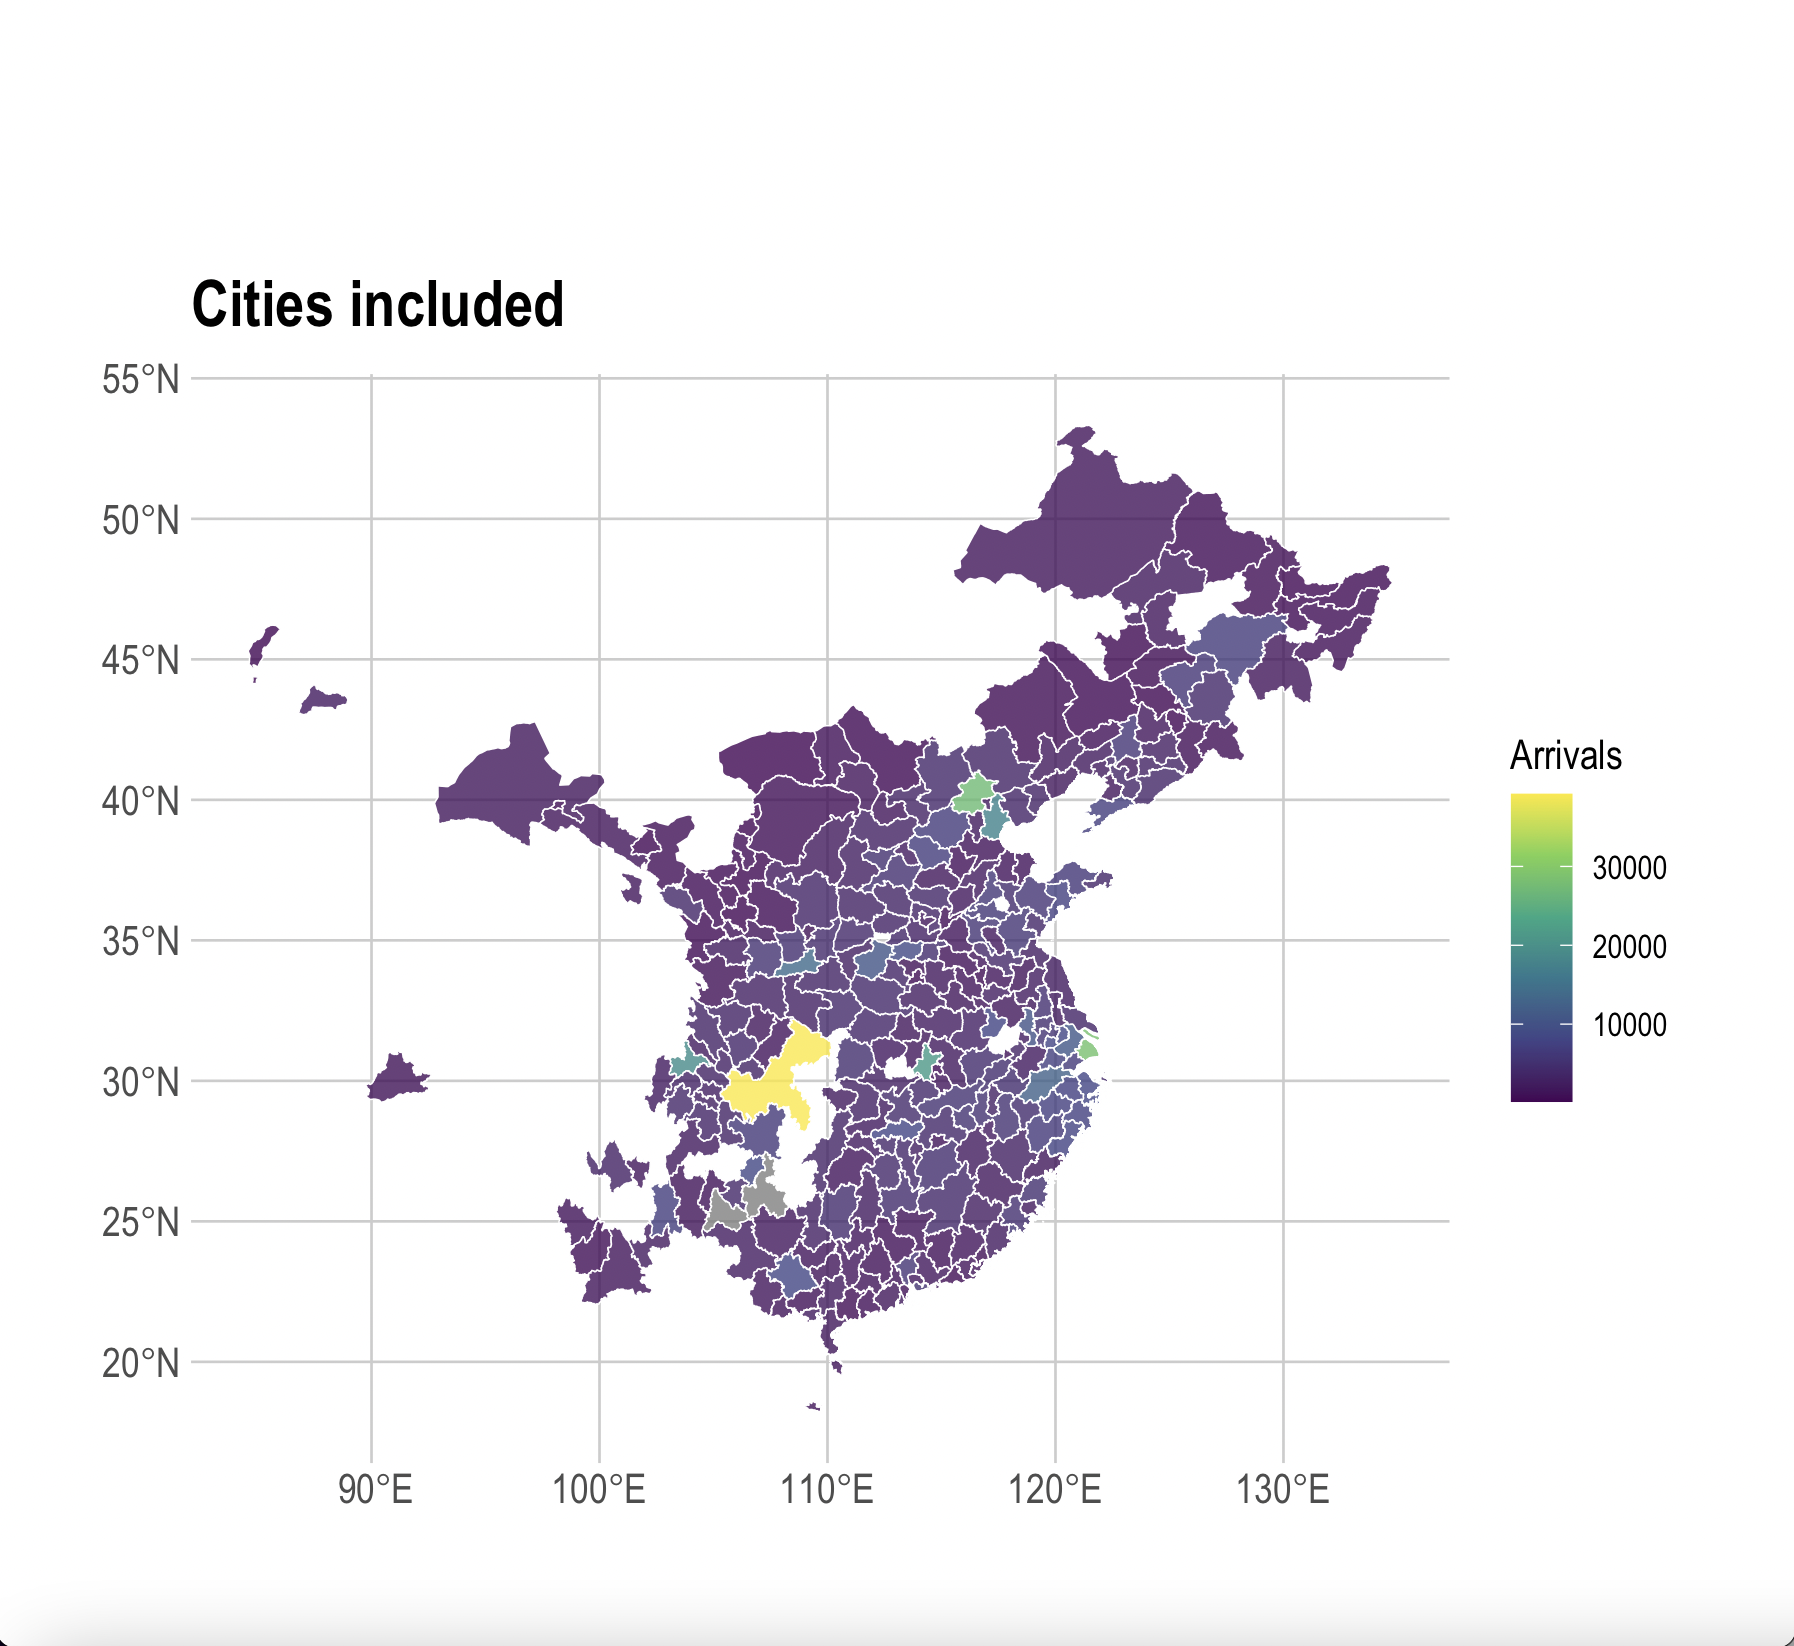
\includegraphics[width=0.5\textwidth,height=\textheight]{/Users/jialiangchen/Documents/spmodeltoruism/figures/figure1.png}

\hypertarget{spatial-autocorrelation-check}{%
\subsection{Spatial Autocorrelation
check}\label{spatial-autocorrelation-check}}

Let's check some Moran's I statistics. Before that, we need to prepare a
list of weights based on neighboring
relationships.\texttt{spdep::poly2nb} produces such neighboring
relationships, and then \texttt{spdep::nb2listw} turns them into
weights.

\begin{Shaded}
\begin{Highlighting}[]
\DocumentationTok{\#\# Use cross{-}sectional data from 2015 for the moment.}
\NormalTok{filter2015 }\OtherTok{\textless{}{-}}\NormalTok{ ct\_spdata\_long }\SpecialCharTok{\%\textgreater{}\%} \FunctionTok{filter}\NormalTok{(year }\SpecialCharTok{==} \DecValTok{2015}\NormalTok{)}
\DocumentationTok{\#\# Create a weighting matrix based on contiguity relations.}
\NormalTok{filter2015 }\SpecialCharTok{\%\textgreater{}\%}\NormalTok{ spdep}\SpecialCharTok{::}\FunctionTok{poly2nb}\NormalTok{(}\StringTok{"geometry"}\NormalTok{) }\SpecialCharTok{\%\textgreater{}\%} 
\NormalTok{  spdep}\SpecialCharTok{::}\FunctionTok{nb2listw}\NormalTok{(}\AttributeTok{zero.policy =} \ConstantTok{TRUE}\NormalTok{) }\OtherTok{{-}\textgreater{}}\NormalTok{ Wnb}
\end{Highlighting}
\end{Shaded}

\hypertarget{global-morans-i-statistics}{%
\subsubsection{Global Moran's I
statistics}\label{global-morans-i-statistics}}

\begin{Shaded}
\begin{Highlighting}[]
\DocumentationTok{\#\# Calculate the Moran\textquotesingle{}s I test with matrix Wnb and year 2015.}
\NormalTok{Wnb }\SpecialCharTok{\%\textgreater{}\%}
\NormalTok{  spdep}\SpecialCharTok{::}\FunctionTok{moran.test}\NormalTok{(filter2015}\SpecialCharTok{$}\NormalTok{tarvl, ., }\AttributeTok{zero.policy =} \ConstantTok{TRUE}\NormalTok{)}
\end{Highlighting}
\end{Shaded}

\begin{verbatim}
## 
##  Moran I test under randomisation
## 
## data:  filter2015$tarvl  
## weights: .  n reduced by no-neighbour observations
##   
## 
## Moran I statistic standard deviate = 4.2406, p-value = 1.115e-05
## alternative hypothesis: greater
## sample estimates:
## Moran I statistic       Expectation          Variance 
##       0.158839281      -0.003636364       0.001468016
\end{verbatim}

The result shows a positive Moran I statistics, as we expected. It is
both substantively (\(\approx 0.16\)) and statistically significant
(with a p-value \(0.00001139\)).

We could try different weighting schemes and different years, but let's
draw a Moran scatter-plot. The solid line in the plot indicates in the
Moran's I statistic. It goes though the mean values and its slope is
exactly the Moran's I.

\begin{Shaded}
\begin{Highlighting}[]
\NormalTok{ spdep}\SpecialCharTok{::}\FunctionTok{moran.plot}\NormalTok{(filter2015}\SpecialCharTok{$}\NormalTok{tarvl, }
\NormalTok{                   Wnb, }
                   \AttributeTok{zero.policy =} \ConstantTok{TRUE}\NormalTok{, }
                   \AttributeTok{xlab =} \StringTok{\textquotesingle{}Total Tourism Arrivals\textquotesingle{}}\NormalTok{,}
                   \AttributeTok{ylab =} \StringTok{\textquotesingle{}Lagged Total Tourism Arrivals (of Neighbors)\textquotesingle{}}\NormalTok{,}
                   \AttributeTok{pch=}\DecValTok{20}\NormalTok{)}
\end{Highlighting}
\end{Shaded}

\includegraphics{spatial_tourism_cn_files/figure-latex/unnamed-chunk-11-1.pdf}

\hypertarget{local-morans-i-statistics}{%
\subsubsection{Local Moran's I
statistics}\label{local-morans-i-statistics}}

We can use Local Moran's I or Local Indicators of Spatial Association
(LISA). LISA can help identify clusters of high or low values as well as
outliers that are surrounded by opposite values.

\begin{Shaded}
\begin{Highlighting}[]
\CommentTok{\# use spdep package to test (global autocorrelation)}
\CommentTok{\# spdep::localmoran, spdep::localmoran.exact}
\CommentTok{\# local moran result: }
\DocumentationTok{\#\#  High positive Ii means simlar values (either high or low clusters)}
\DocumentationTok{\#\#  Low negative Ii means dissimilar values (outliers)}
\DocumentationTok{\#\#  }

\NormalTok{lisaRslt }\OtherTok{\textless{}{-}}\NormalTok{ spdep}\SpecialCharTok{::}\FunctionTok{localmoran}\NormalTok{(filter2015}\SpecialCharTok{$}\NormalTok{tarvl, Wnb, }
                              \AttributeTok{zero.policy =} \ConstantTok{TRUE}\NormalTok{, }\AttributeTok{na.action =}\NormalTok{ na.omit)}

\DocumentationTok{\#\# The dimension of LISA result and the orignal sf object}
\FunctionTok{dim}\NormalTok{(lisaRslt)}
\end{Highlighting}
\end{Shaded}

\begin{verbatim}
## [1] 283   5
\end{verbatim}

\begin{Shaded}
\begin{Highlighting}[]
\FunctionTok{dim}\NormalTok{(filter2015)}
\end{Highlighting}
\end{Shaded}

\begin{verbatim}
## [1] 283  25
\end{verbatim}

\begin{Shaded}
\begin{Highlighting}[]
\DocumentationTok{\#\# Show some of the results.}
\FunctionTok{head}\NormalTok{(lisaRslt)}
\end{Highlighting}
\end{Shaded}

\begin{verbatim}
##            Ii          E.Ii      Var.Ii       Z.Ii Pr(z != E(Ii))
## 1 -0.01565477 -0.0002340732 0.013056893 -0.1349535      0.8926487
## 2  0.10086269 -0.0001412031 0.006540647  1.2489003      0.2117015
## 3  0.21416980 -0.0008064452 0.037330384  1.1126517      0.2658580
## 4  0.01720986 -0.0003042559 0.010491739  0.1709875      0.8642336
## 5 -0.09950736 -0.0006569431 0.025975094 -0.6133381      0.5396528
## 6  0.13076504 -0.0005635281 0.026092081  0.8130268      0.4162027
\end{verbatim}

Note that \texttt{Ii} stands for the local moran statistic,
\texttt{E.Ii} is the expectation of local moran statistic,
\texttt{Var.Ii} is the variance, \texttt{Z.Ii} is the standard
deviation, and \texttt{Pr(z\ \textgreater{}\ 0)} is the p-values.

Assuming statistical significance, if \(\text{Ii} > 0\), it would be a
cluster (similar to nearby or neighboring values, HH or LL); if
\(\text{Ii} < 0\), it would be a outlier (very different from nearby or
neighboring values, HL or LH).

\begin{Shaded}
\begin{Highlighting}[]
\CommentTok{\# Now we can derive the cluster/outlier types for each spatial feature in the data}
\NormalTok{significanceLevel }\OtherTok{\textless{}{-}} \FloatTok{0.05} \CommentTok{\# 95\% confidence}
\NormalTok{meanVal }\OtherTok{\textless{}{-}} \FunctionTok{mean}\NormalTok{(filter2015}\SpecialCharTok{$}\NormalTok{tarvl)}

\NormalTok{lisaRslt }\SpecialCharTok{\%\textless{}\textgreater{}\%}\NormalTok{ tibble}\SpecialCharTok{::}\FunctionTok{as\_tibble}\NormalTok{() }\SpecialCharTok{\%\textgreater{}\%}
\NormalTok{  magrittr}\SpecialCharTok{::}\FunctionTok{set\_colnames}\NormalTok{(}\FunctionTok{c}\NormalTok{(}\StringTok{"Ii"}\NormalTok{,}\StringTok{"E.Ii"}\NormalTok{,}\StringTok{"Var.Ii"}\NormalTok{,}\StringTok{"Z.Ii"}\NormalTok{,}\StringTok{"Pr(z \textgreater{} 0)"}\NormalTok{)) }\SpecialCharTok{\%\textgreater{}\%}
\NormalTok{  dplyr}\SpecialCharTok{::}\FunctionTok{mutate}\NormalTok{(}\AttributeTok{coType =}\NormalTok{ dplyr}\SpecialCharTok{::}\FunctionTok{case\_when}\NormalTok{(}
  \StringTok{\textasciigrave{}}\AttributeTok{Pr(z \textgreater{} 0)}\StringTok{\textasciigrave{}} \SpecialCharTok{\textgreater{}} \FloatTok{0.05} \SpecialCharTok{\textasciitilde{}} \StringTok{"Insignificant"}\NormalTok{,}
  \StringTok{\textasciigrave{}}\AttributeTok{Pr(z \textgreater{} 0)}\StringTok{\textasciigrave{}} \SpecialCharTok{\textless{}=} \FloatTok{0.05} \SpecialCharTok{\&}\NormalTok{ Ii }\SpecialCharTok{\textgreater{}=} \DecValTok{0} \SpecialCharTok{\&}\NormalTok{ filter2015}\SpecialCharTok{$}\NormalTok{tarvl }\SpecialCharTok{\textgreater{}=}\NormalTok{ meanVal }\SpecialCharTok{\textasciitilde{}} \StringTok{"HH"}\NormalTok{,}
  \StringTok{\textasciigrave{}}\AttributeTok{Pr(z \textgreater{} 0)}\StringTok{\textasciigrave{}} \SpecialCharTok{\textless{}=} \FloatTok{0.05} \SpecialCharTok{\&}\NormalTok{ Ii }\SpecialCharTok{\textgreater{}=} \DecValTok{0} \SpecialCharTok{\&}\NormalTok{ filter2015}\SpecialCharTok{$}\NormalTok{tarvl }\SpecialCharTok{\textless{}}\NormalTok{ meanVal }\SpecialCharTok{\textasciitilde{}} \StringTok{"LL"}\NormalTok{,}
  \StringTok{\textasciigrave{}}\AttributeTok{Pr(z \textgreater{} 0)}\StringTok{\textasciigrave{}} \SpecialCharTok{\textless{}=} \FloatTok{0.05} \SpecialCharTok{\&}\NormalTok{ Ii }\SpecialCharTok{\textless{}} \DecValTok{0} \SpecialCharTok{\&}\NormalTok{ filter2015}\SpecialCharTok{$}\NormalTok{tarvl }\SpecialCharTok{\textgreater{}=}\NormalTok{ meanVal }\SpecialCharTok{\textasciitilde{}} \StringTok{"HL"}\NormalTok{,}
  \StringTok{\textasciigrave{}}\AttributeTok{Pr(z \textgreater{} 0)}\StringTok{\textasciigrave{}} \SpecialCharTok{\textless{}=} \FloatTok{0.05} \SpecialCharTok{\&}\NormalTok{ Ii }\SpecialCharTok{\textless{}} \DecValTok{0} \SpecialCharTok{\&}\NormalTok{ filter2015}\SpecialCharTok{$}\NormalTok{tarvl }\SpecialCharTok{\textless{}}\NormalTok{ meanVal }\SpecialCharTok{\textasciitilde{}} \StringTok{"LH"}
\NormalTok{))}

\CommentTok{\# Now add this coType to original sf data}
\NormalTok{filter2015}\SpecialCharTok{$}\NormalTok{coType }\OtherTok{\textless{}{-}}\NormalTok{ lisaRslt}\SpecialCharTok{$}\NormalTok{coType }\SpecialCharTok{\%\textgreater{}\%}\NormalTok{ tidyr}\SpecialCharTok{::}\FunctionTok{replace\_na}\NormalTok{(}\StringTok{"Insignificant"}\NormalTok{)}

\FunctionTok{ggplot}\NormalTok{(filter2015) }\SpecialCharTok{+}
  \FunctionTok{geom\_sf}\NormalTok{(}\FunctionTok{aes}\NormalTok{(}\AttributeTok{fill=}\NormalTok{coType),}\AttributeTok{color =} \StringTok{\textquotesingle{}lightgrey\textquotesingle{}}\NormalTok{) }\SpecialCharTok{+}
  \FunctionTok{scale\_fill\_manual}\NormalTok{(}\AttributeTok{values =} \FunctionTok{c}\NormalTok{(}\StringTok{\textquotesingle{}red\textquotesingle{}}\NormalTok{,}\StringTok{\textquotesingle{}brown\textquotesingle{}}\NormalTok{,}\StringTok{\textquotesingle{}green\textquotesingle{}}\NormalTok{,}\StringTok{\textquotesingle{}blue\textquotesingle{}}\NormalTok{,}\StringTok{\textquotesingle{}cyan\textquotesingle{}}\NormalTok{), }\AttributeTok{name=}\StringTok{\textquotesingle{}Clusters \& }\SpecialCharTok{\textbackslash{}n}\StringTok{Outliers\textquotesingle{}}\NormalTok{) }\SpecialCharTok{+}
  \FunctionTok{labs}\NormalTok{(}\AttributeTok{title =} \StringTok{"Tourism arrivals of our included cities, year2015"}\NormalTok{)}
\end{Highlighting}
\end{Shaded}

\includegraphics{spatial_tourism_cn_files/figure-latex/unnamed-chunk-13-1.pdf}

\hypertarget{spatial-corss-sectional-regressions}{%
\subsection{Spatial Corss-sectional
regressions}\label{spatial-corss-sectional-regressions}}

\hypertarget{spatial-error-model}{%
\subsubsection{Spatial Error Model}\label{spatial-error-model}}

As a point of departure, we do an OLS and test whether spatial
autocorrelation is present in the residuals.

\begin{Shaded}
\begin{Highlighting}[]
\NormalTok{olsRslt }\OtherTok{\textless{}{-}} \FunctionTok{lm}\NormalTok{(}\FunctionTok{log}\NormalTok{(tarvl}\SpecialCharTok{+}\DecValTok{1}\NormalTok{) }\SpecialCharTok{\textasciitilde{}}\NormalTok{ CPIp }\SpecialCharTok{+}
                \FunctionTok{log}\NormalTok{(}\DecValTok{1}\SpecialCharTok{+}\NormalTok{salary) }\SpecialCharTok{+}
                \FunctionTok{log}\NormalTok{(}\DecValTok{1}\SpecialCharTok{+}\NormalTok{area) }\SpecialCharTok{+} \FunctionTok{log}\NormalTok{(}\DecValTok{1}\SpecialCharTok{+}\NormalTok{pop) }\SpecialCharTok{+}
                \FunctionTok{log}\NormalTok{(}\DecValTok{1}\SpecialCharTok{+}\NormalTok{railway),}
              \AttributeTok{data =}\NormalTok{ filter2015,)}
\FunctionTok{summary}\NormalTok{(olsRslt)}
\end{Highlighting}
\end{Shaded}

\begin{verbatim}
## 
## Call:
## lm(formula = log(tarvl + 1) ~ CPIp + log(1 + salary) + log(1 + 
##     area) + log(1 + pop) + log(1 + railway), data = filter2015)
## 
## Residuals:
##     Min      1Q  Median      3Q     Max 
## -1.9460 -0.4161  0.0958  0.4460  1.4085 
## 
## Coefficients:
##                  Estimate Std. Error t value Pr(>|t|)    
## (Intercept)      -7.57701    8.57218  -0.884 0.377516    
## CPIp              0.01980    0.08097   0.245 0.807009    
## log(1 + salary)   0.89030    0.24806   3.589 0.000393 ***
## log(1 + area)    -0.07020    0.04784  -1.467 0.143401    
## log(1 + pop)      0.72566    0.06373  11.387  < 2e-16 ***
## log(1 + railway)  0.09363    0.04342   2.156 0.031917 *  
## ---
## Signif. codes:  0 '***' 0.001 '**' 0.01 '*' 0.05 '.' 0.1 ' ' 1
## 
## Residual standard error: 0.6342 on 276 degrees of freedom
##   (1 observation deleted due to missingness)
## Multiple R-squared:  0.5006, Adjusted R-squared:  0.4916 
## F-statistic: 55.34 on 5 and 276 DF,  p-value: < 2.2e-16
\end{verbatim}

\begin{Shaded}
\begin{Highlighting}[]
\CommentTok{\# Derive the residuals from the regression. Need to handle those missed values.}
\NormalTok{lmResiduals }\OtherTok{\textless{}{-}} \FunctionTok{rep}\NormalTok{(}\DecValTok{0}\NormalTok{, }\FunctionTok{length}\NormalTok{(filter2015}\SpecialCharTok{$}\NormalTok{tarvl)) }\CommentTok{\#create a bunch of zeros}
\NormalTok{resIndex }\OtherTok{\textless{}{-}}\NormalTok{ olsRslt}\SpecialCharTok{$}\NormalTok{residuals }\SpecialCharTok{\%\textgreater{}\%} \FunctionTok{names}\NormalTok{() }\SpecialCharTok{\%\textgreater{}\%} \FunctionTok{as.integer}\NormalTok{() }\CommentTok{\#create index for our 283 residuals}
\NormalTok{lmResiduals[resIndex] }\OtherTok{\textless{}{-}}\NormalTok{ olsRslt}\SpecialCharTok{$}\NormalTok{residuals}

\CommentTok{\# Test if there is spatial autocorrelation in the regression residuals (errors).}
\NormalTok{Wnb }\SpecialCharTok{\%\textgreater{}\%}
\NormalTok{  spdep}\SpecialCharTok{::}\FunctionTok{moran.test}\NormalTok{(lmResiduals, ., }\AttributeTok{zero.policy =} \ConstantTok{TRUE}\NormalTok{)}
\end{Highlighting}
\end{Shaded}

\begin{verbatim}
## 
##  Moran I test under randomisation
## 
## data:  lmResiduals  
## weights: .  n reduced by no-neighbour observations
##   
## 
## Moran I statistic standard deviate = 11.417, p-value < 2.2e-16
## alternative hypothesis: greater
## sample estimates:
## Moran I statistic       Expectation          Variance 
##       0.460466806      -0.003636364       0.001652481
\end{verbatim}

Our result show statistically and economically significant Moran I
statistic, which implies that the residuals from linear regression have
positive spatial autocorrelation. With that, we do a SAR error model.

\[Y = X\beta + u, \qquad \text{where} \quad u = \lambda Wu + \epsilon.\]

\begin{Shaded}
\begin{Highlighting}[]
\CommentTok{\# use spdep package to run the spatial error model }
\CommentTok{\# Use spatialreg::errorsarlm to run the same model}
\NormalTok{serrRslt }\OtherTok{\textless{}{-}}\NormalTok{ spatialreg}\SpecialCharTok{::}\FunctionTok{errorsarlm}\NormalTok{(}\FunctionTok{log}\NormalTok{(tarvl}\SpecialCharTok{+}\DecValTok{1}\NormalTok{) }\SpecialCharTok{\textasciitilde{}}\NormalTok{ CPIp }\SpecialCharTok{+}
                \FunctionTok{log}\NormalTok{(}\DecValTok{1}\SpecialCharTok{+}\NormalTok{salary) }\SpecialCharTok{+}
                \FunctionTok{log}\NormalTok{(}\DecValTok{1}\SpecialCharTok{+}\NormalTok{area) }\SpecialCharTok{+} \FunctionTok{log}\NormalTok{(}\DecValTok{1}\SpecialCharTok{+}\NormalTok{pop) }\SpecialCharTok{+}
                \FunctionTok{log}\NormalTok{(}\DecValTok{1}\SpecialCharTok{+}\NormalTok{railway),}
              \AttributeTok{data =}\NormalTok{ filter2015,}
              \AttributeTok{listw =}\NormalTok{ Wnb,}
              \CommentTok{\# Durbin = TRUE, \#uncomment for including lagged X}
              \AttributeTok{zero.policy =} \ConstantTok{TRUE}\NormalTok{, }
              \AttributeTok{na.action =}\NormalTok{ na.omit);}

\FunctionTok{summary}\NormalTok{(serrRslt)}
\end{Highlighting}
\end{Shaded}

\begin{verbatim}
## 
## Call:spatialreg::errorsarlm(formula = log(tarvl + 1) ~ CPIp + log(1 + 
##     salary) + log(1 + area) + log(1 + pop) + log(1 + railway), 
##     data = filter2015, listw = Wnb, na.action = na.omit, zero.policy = TRUE)
## 
## Residuals:
##       Min        1Q    Median        3Q       Max 
## -1.538731 -0.281105  0.020747  0.355871  1.037318 
## 
## Type: error 
## Regions with no neighbours included:
##  79 80 202 260 261 262 281 
## Coefficients: (asymptotic standard errors) 
##                   Estimate Std. Error z value  Pr(>|z|)
## (Intercept)      -7.984165   6.607437 -1.2084   0.22691
## CPIp              0.010112   0.060373  0.1675   0.86699
## log(1 + salary)   0.991205   0.238479  4.1564 3.233e-05
## log(1 + area)    -0.018311   0.047274 -0.3873   0.69851
## log(1 + pop)      0.689489   0.062013 11.1184 < 2.2e-16
## log(1 + railway)  0.067681   0.033039  2.0485   0.04051
## 
## Lambda: 0.67767, LR test value: 112.1, p-value: < 2.22e-16
## Asymptotic standard error: 0.049473
##     z-value: 13.698, p-value: < 2.22e-16
## Wald statistic: 187.63, p-value: < 2.22e-16
## 
## Log likelihood: -212.6233 for error model
## ML residual variance (sigma squared): 0.23265, (sigma: 0.48234)
## Number of observations: 282 
## Number of parameters estimated: 8 
## AIC: 441.25, (AIC for lm: 551.34)
\end{verbatim}

From the AIC, the spatial error model performs better than the linear
model. Now we test if there is spatial dependence left after we
controled that for the error term.

\begin{Shaded}
\begin{Highlighting}[]
\CommentTok{\# Derive the residuals from the regression. Need to handle those missed values.}
\NormalTok{seResiduals }\OtherTok{\textless{}{-}} \FunctionTok{rep}\NormalTok{(}\DecValTok{0}\NormalTok{, }\FunctionTok{length}\NormalTok{(filter2015}\SpecialCharTok{$}\NormalTok{tarvl))}
\NormalTok{resIndex }\OtherTok{\textless{}{-}}\NormalTok{ serrRslt}\SpecialCharTok{$}\NormalTok{residuals }\SpecialCharTok{\%\textgreater{}\%} \FunctionTok{names}\NormalTok{() }\SpecialCharTok{\%\textgreater{}\%} \FunctionTok{as.integer}\NormalTok{();}
\NormalTok{seResiduals[resIndex] }\OtherTok{\textless{}{-}}\NormalTok{ serrRslt}\SpecialCharTok{$}\NormalTok{residuals}

\CommentTok{\# Test if there is spatial autocorrelation in the regression residuals (errors).}
\NormalTok{Wnb }\SpecialCharTok{\%\textgreater{}\%}
\NormalTok{  spdep}\SpecialCharTok{::}\FunctionTok{moran.test}\NormalTok{(seResiduals, ., }\AttributeTok{zero.policy =} \ConstantTok{TRUE}\NormalTok{) }
\end{Highlighting}
\end{Shaded}

\begin{verbatim}
## 
##  Moran I test under randomisation
## 
## data:  seResiduals  
## weights: .  n reduced by no-neighbour observations
##   
## 
## Moran I statistic standard deviate = -0.11335, p-value = 0.5451
## alternative hypothesis: greater
## sample estimates:
## Moran I statistic       Expectation          Variance 
##      -0.008241803      -0.003636364       0.001650706
\end{verbatim}

We cannot reject the null. We are good to go.

\hypertarget{spatial-lag-model}{%
\subsubsection{Spatial Lag Model}\label{spatial-lag-model}}

This time, we estimate the following model, aka. The spatial lag model.
\[Y = \rho WY + X\beta + \epsilon.\]

\begin{Shaded}
\begin{Highlighting}[]
\CommentTok{\# use spdep package to run the spatial lag model }
\CommentTok{\# spatialreg::lagsarlm }
\NormalTok{slmRslt }\OtherTok{\textless{}{-}}\NormalTok{ spatialreg}\SpecialCharTok{::}\FunctionTok{lagsarlm}\NormalTok{(}\FunctionTok{log}\NormalTok{(tarvl}\SpecialCharTok{+}\DecValTok{1}\NormalTok{) }\SpecialCharTok{\textasciitilde{}}\NormalTok{ CPIp }\SpecialCharTok{+}
                \FunctionTok{log}\NormalTok{(}\DecValTok{1}\SpecialCharTok{+}\NormalTok{salary) }\SpecialCharTok{+}
                \FunctionTok{log}\NormalTok{(}\DecValTok{1}\SpecialCharTok{+}\NormalTok{area) }\SpecialCharTok{+} \FunctionTok{log}\NormalTok{(}\DecValTok{1}\SpecialCharTok{+}\NormalTok{pop) }\SpecialCharTok{+}
                \FunctionTok{log}\NormalTok{(}\DecValTok{1}\SpecialCharTok{+}\NormalTok{railway),}
              \AttributeTok{data =}\NormalTok{ filter2015,}
              \AttributeTok{listw =}\NormalTok{ Wnb,}
              \CommentTok{\# Durbin = TRUE, \#uncomment for including lagged X}
              \AttributeTok{zero.policy =} \ConstantTok{TRUE}\NormalTok{, }
              \AttributeTok{na.action =}\NormalTok{ na.omit);}

\FunctionTok{summary}\NormalTok{(slmRslt)}
\end{Highlighting}
\end{Shaded}

\begin{verbatim}
## 
## Call:spatialreg::lagsarlm(formula = log(tarvl + 1) ~ CPIp + log(1 + 
##     salary) + log(1 + area) + log(1 + pop) + log(1 + railway), 
##     data = filter2015, listw = Wnb, na.action = na.omit, zero.policy = TRUE)
## 
## Residuals:
##      Min       1Q   Median       3Q      Max 
## -1.83395 -0.40452  0.10717  0.43161  1.73382 
## 
## Type: lag 
## Regions with no neighbours included:
##  79 80 202 260 261 262 281 
## Coefficients: (asymptotic standard errors) 
##                    Estimate Std. Error z value  Pr(>|z|)
## (Intercept)      -10.774585   8.172903 -1.3183   0.18739
## CPIp               0.014675   0.077028  0.1905   0.84890
## log(1 + salary)    1.181143   0.242473  4.8712 1.109e-06
## log(1 + area)     -0.059298   0.045542 -1.3021   0.19290
## log(1 + pop)       0.629619   0.064312  9.7901 < 2.2e-16
## log(1 + railway)   0.083422   0.041312  2.0193   0.04346
## 
## Rho: 0.1336, LR test value: 21.083, p-value: 4.3988e-06
## Asymptotic standard error: 0.029262
##     z-value: 4.5656, p-value: 4.9797e-06
## Wald statistic: 20.845, p-value: 4.9797e-06
## 
## Log likelihood: -258.1296 for lag model
## ML residual variance (sigma squared): 0.36383, (sigma: 0.60318)
## Number of observations: 282 
## Number of parameters estimated: 8 
## AIC: 532.26, (AIC for lm: 551.34)
## LM test for residual autocorrelation
## test value: 97.842, p-value: < 2.22e-16
\end{verbatim}

We can also calculate the direct, indirect and total impacts.

\begin{Shaded}
\begin{Highlighting}[]
\NormalTok{trMnb }\OtherTok{\textless{}{-}} \FunctionTok{trW}\NormalTok{(}\AttributeTok{listw =}\NormalTok{ Wnb, }\AttributeTok{type=} \StringTok{"moments"}\NormalTok{)}
\FunctionTok{impacts}\NormalTok{(slmRslt, }\AttributeTok{tr =}\NormalTok{ trMnb)}
\end{Highlighting}
\end{Shaded}

\begin{verbatim}
## Impact measures (lag, trace):
##                       Direct     Indirect       Total
## CPIp              0.01474136  0.002197074  0.01693844
## log(1 + salary)   1.18644910  0.176830051  1.36327915
## log(1 + area)    -0.05956448 -0.008877575 -0.06844206
## log(1 + pop)      0.63244755  0.094260877  0.72670843
## log(1 + railway)  0.08379653  0.012489153  0.09628568
\end{verbatim}

The spatial lag term \(\rho\) is highly statistically and economically
significant (greater than \(0\)).

\begin{Shaded}
\begin{Highlighting}[]
\CommentTok{\# Derive the residuals from the regression. Need to handle those missed values}
\NormalTok{slResiduals }\OtherTok{\textless{}{-}} \FunctionTok{rep}\NormalTok{(}\DecValTok{0}\NormalTok{, }\FunctionTok{length}\NormalTok{(filter2015}\SpecialCharTok{$}\NormalTok{tarvl))}
\NormalTok{resIndex }\OtherTok{\textless{}{-}}\NormalTok{ slmRslt}\SpecialCharTok{$}\NormalTok{residuals }\SpecialCharTok{\%\textgreater{}\%} \FunctionTok{names}\NormalTok{() }\SpecialCharTok{\%\textgreater{}\%} \FunctionTok{as.integer}\NormalTok{();}
\NormalTok{slResiduals[resIndex] }\OtherTok{\textless{}{-}}\NormalTok{ slmRslt}\SpecialCharTok{$}\NormalTok{residuals}

\CommentTok{\# Test if there is spatial autocorrelation in the regression residuals (errors) after we corrected the spatial dependence by including the spatially lagged dependent variable.}
\NormalTok{Wnb }\SpecialCharTok{\%\textgreater{}\%}
\NormalTok{  spdep}\SpecialCharTok{::}\FunctionTok{moran.test}\NormalTok{(slResiduals, ., }\AttributeTok{zero.policy =} \ConstantTok{TRUE}\NormalTok{)}
\end{Highlighting}
\end{Shaded}

\begin{verbatim}
## 
##  Moran I test under randomisation
## 
## data:  slResiduals  
## weights: .  n reduced by no-neighbour observations
##   
## 
## Moran I statistic standard deviate = 9.2614, p-value < 2.2e-16
## alternative hypothesis: greater
## sample estimates:
## Moran I statistic       Expectation          Variance 
##       0.372705782      -0.003636364       0.001651233
\end{verbatim}

\hypertarget{sarar-model}{%
\subsubsection{SARAR model}\label{sarar-model}}

There is\ldots, but let's run a ``SAC/SARAR'' model.
\[y = \rho Wy + X\beta + u, \qquad\text{where}\quad u = \lambda Wu + \epsilon.\]

\begin{Shaded}
\begin{Highlighting}[]
\CommentTok{\# use spdep package to run the spatial lag and spatial error model }
\CommentTok{\# spatialreg::sacsarlm}
\NormalTok{sararRslt }\OtherTok{\textless{}{-}}\NormalTok{ spatialreg}\SpecialCharTok{::}\FunctionTok{sacsarlm}\NormalTok{(}\FunctionTok{log}\NormalTok{(tarvl}\SpecialCharTok{+}\DecValTok{1}\NormalTok{) }\SpecialCharTok{\textasciitilde{}}\NormalTok{ CPIp }\SpecialCharTok{+}
                \FunctionTok{log}\NormalTok{(}\DecValTok{1}\SpecialCharTok{+}\NormalTok{salary) }\SpecialCharTok{+}
                \FunctionTok{log}\NormalTok{(}\DecValTok{1}\SpecialCharTok{+}\NormalTok{area) }\SpecialCharTok{+} \FunctionTok{log}\NormalTok{(}\DecValTok{1}\SpecialCharTok{+}\NormalTok{pop) }\SpecialCharTok{+}
                \FunctionTok{log}\NormalTok{(}\DecValTok{1}\SpecialCharTok{+}\NormalTok{railway),}
              \AttributeTok{data =}\NormalTok{ filter2015,}
              \AttributeTok{listw =}\NormalTok{ Wnb,}
              \CommentTok{\# Durbin = TRUE, \#uncomment for including lagged X}
              \AttributeTok{zero.policy =} \ConstantTok{TRUE}\NormalTok{,}
              \AttributeTok{na.action =}\NormalTok{ na.omit)}

\FunctionTok{summary}\NormalTok{(sararRslt)}
\end{Highlighting}
\end{Shaded}

\begin{verbatim}
## 
## Call:spatialreg::sacsarlm(formula = log(tarvl + 1) ~ CPIp + log(1 + 
##     salary) + log(1 + area) + log(1 + pop) + log(1 + railway), 
##     data = filter2015, listw = Wnb, na.action = na.omit, zero.policy = TRUE)
## 
## Residuals:
##       Min        1Q    Median        3Q       Max 
## -1.542667 -0.292160  0.014007  0.348345  1.045453 
## 
## Type: sac 
## Coefficients: (asymptotic standard errors) 
##                   Estimate Std. Error z value  Pr(>|z|)
## (Intercept)      -8.800575   6.729588 -1.3077   0.19096
## CPIp              0.010499   0.060565  0.1734   0.86237
## log(1 + salary)   1.054582   0.258254  4.0835 4.436e-05
## log(1 + area)    -0.017537   0.047246 -0.3712   0.71050
## log(1 + pop)      0.682788   0.062998 10.8382 < 2.2e-16
## log(1 + railway)  0.065354   0.033318  1.9615   0.04982
## 
## Rho: 0.018297
## Asymptotic standard error: 0.027837
##     z-value: 0.6573, p-value: 0.51099
## Lambda: 0.66699
## Asymptotic standard error: 0.052657
##     z-value: 12.667, p-value: < 2.22e-16
## 
## LR test value: 112.53, p-value: < 2.22e-16
## 
## Log likelihood: -212.4074 for sac model
## ML residual variance (sigma squared): 0.23345, (sigma: 0.48316)
## Number of observations: 282 
## Number of parameters estimated: 9 
## AIC: 442.81, (AIC for lm: 551.34)
\end{verbatim}

\hypertarget{spatial-panel-regressions}{%
\subsection{Spatial panel regressions}\label{spatial-panel-regressions}}

\hypertarget{preparation}{%
\subsubsection{Preparation}\label{preparation}}

My feeling is that panel data are sensitive to NAs and empty
neighborhoods in R. With that, I will first construct a new weighting
matrix W, and then deal with the NAs in our data.

Take a look of our where do our NAs inhabit.

\begin{Shaded}
\begin{Highlighting}[]
\FunctionTok{which}\NormalTok{(ct\_spdata\_long }\SpecialCharTok{\%\textgreater{}\%} \FunctionTok{is.na}\NormalTok{()  }\SpecialCharTok{\%\textgreater{}\%} \FunctionTok{colSums}\NormalTok{() }\SpecialCharTok{\textgreater{}} \DecValTok{0}\NormalTok{) }\SpecialCharTok{\%\textgreater{}\%} \FunctionTok{names}\NormalTok{()}
\end{Highlighting}
\end{Shaded}

\begin{verbatim}
##  [1] "hprice" "pgdp"   "salary" "pop"    "area"   "road"   "hotel"  "agent" 
##  [9] "Aspot"  "darvl"  "irev"
\end{verbatim}

Take a look of our old weighting scheme (Recall that it was based on
continguity).

\begin{Shaded}
\begin{Highlighting}[]
\FunctionTok{summary}\NormalTok{(Wnb, }\AttributeTok{zero.policy=}\ConstantTok{TRUE}\NormalTok{)}
\end{Highlighting}
\end{Shaded}

\begin{verbatim}
## Characteristics of weights list object:
## Neighbour list object:
## Number of regions: 283 
## Number of nonzero links: 1362 
## Percentage nonzero weights: 1.700608 
## Average number of links: 4.812721 
## 7 regions with no links:
## 79 80 202 260 261 262 281
## Link number distribution:
## 
##  0  1  2  3  4  5  6  7  8  9 10 
##  7  4 28 33 44 52 68 26 13  7  1 
## 4 least connected regions:
## 225 253 263 265 with 1 link
## 1 most connected region:
## 238 with 10 links
## 
## Weights style: W 
## Weights constants summary:
##     n    nn  S0       S1       S2
## W 276 76176 276 128.0013 1140.501
\end{verbatim}

As you can see, there are 7 regions with no links: 79(海口) 80(三亚)
202(西宁) 260(乌鲁木齐) 261(克拉玛依) 262(拉萨) 281(舟山). We should
deal with these two problems in turn.

\hypertarget{nearest-neighbors-weighting-matrix}{%
\paragraph{4 Nearest Neighbors Weighting
matrix}\label{nearest-neighbors-weighting-matrix}}

To avoid islands, we contruct a new meighting matrix by 4 NN.

\begin{Shaded}
\begin{Highlighting}[]
\DocumentationTok{\#\# Identify coordinates}
\NormalTok{coords }\OtherTok{\textless{}{-}} \FunctionTok{cbind}\NormalTok{(ct\_data}\SpecialCharTok{$}\NormalTok{Long, ct\_data}\SpecialCharTok{$}\NormalTok{Lat)}

\DocumentationTok{\#\# Create our 4 NN matrix}
\DocumentationTok{\#\# Note that the latitude and longitude are handled using great circle distances}
\DocumentationTok{\#\# R2 distances will be inaccurate}
\NormalTok{matrix5nn }\OtherTok{\textless{}{-}} \FunctionTok{knearneigh}\NormalTok{(coords, }\AttributeTok{k =} \DecValTok{4}\NormalTok{, }\AttributeTok{longlat =} \ConstantTok{TRUE}\NormalTok{)}

\DocumentationTok{\#\# Convert our weighting matrix to neighborhood list}
\NormalTok{W5nnb }\OtherTok{\textless{}{-}} \FunctionTok{knn2nb}\NormalTok{(matrix5nn)}
\DocumentationTok{\#\# Plot the neighborhood relationships}
\FunctionTok{plot}\NormalTok{(W5nnb, coords)}
\end{Highlighting}
\end{Shaded}

\includegraphics{spatial_tourism_cn_files/figure-latex/unnamed-chunk-24-1.pdf}

\begin{Shaded}
\begin{Highlighting}[]
\DocumentationTok{\#\# Convert our neighborhood list to an listw object}
\NormalTok{W5nnlistw }\OtherTok{\textless{}{-}}\NormalTok{ spdep}\SpecialCharTok{::}\FunctionTok{nb2listw}\NormalTok{(W5nnb, }\AttributeTok{zero.policy =} \ConstantTok{FALSE}\NormalTok{) }
\end{Highlighting}
\end{Shaded}

\hypertarget{interpolate-the-missing-values}{%
\paragraph{Interpolate the missing
values}\label{interpolate-the-missing-values}}

We do our interpolation by simple(crude?) linear interpolation. This
actually make sense since in our \texttt{ct\_spdata\_long} dataset, most
of the cities are arranged based on their provinces, also we have nine
time periods for each city. Linear interpolationThey should be fine
because of the geographical similarity and time trends.

\begin{Shaded}
\begin{Highlighting}[]
\DocumentationTok{\#\# We only interpolate the variables we will be using in this document}
\DocumentationTok{\#\# library(zoo)}
\NormalTok{ct\_spdata\_long }\OtherTok{\textless{}{-}}\NormalTok{ ct\_spdata\_long }\SpecialCharTok{\%\textgreater{}\%}
        \FunctionTok{mutate}\NormalTok{(}\AttributeTok{CPIp =} \FunctionTok{na.approx}\NormalTok{(CPIp), }\AttributeTok{salary =} \FunctionTok{na.approx}\NormalTok{(salary), }\AttributeTok{area =} \FunctionTok{na.approx}\NormalTok{(area), }\AttributeTok{pop =} \FunctionTok{na.approx}\NormalTok{(pop), }\AttributeTok{railway =} \FunctionTok{na.approx}\NormalTok{(railway))}
\end{Highlighting}
\end{Shaded}

\hypertarget{spatial-lag-panel-model}{%
\subsubsection{Spatial Lag panel model}\label{spatial-lag-panel-model}}

Since we changed the weighting scheme and did an interpolation, the
following result is not directly comparable with the corss-sectional
results above.

\begin{Shaded}
\begin{Highlighting}[]
\DocumentationTok{\#\# random effects panel with spatial lag}
\NormalTok{sar\_panel }\OtherTok{\textless{}{-}} \FunctionTok{spml}\NormalTok{(}\FunctionTok{log}\NormalTok{(tarvl}\SpecialCharTok{+}\DecValTok{1}\NormalTok{) }\SpecialCharTok{\textasciitilde{}}\NormalTok{ CPIp }\SpecialCharTok{+}
                \FunctionTok{log}\NormalTok{(}\DecValTok{1}\SpecialCharTok{+}\NormalTok{salary) }\SpecialCharTok{+}
                \FunctionTok{log}\NormalTok{(}\DecValTok{1}\SpecialCharTok{+}\NormalTok{area) }\SpecialCharTok{+} \FunctionTok{log}\NormalTok{(}\DecValTok{1}\SpecialCharTok{+}\NormalTok{pop) }\SpecialCharTok{+}
                \FunctionTok{log}\NormalTok{(}\DecValTok{1}\SpecialCharTok{+}\NormalTok{railway),}
               \AttributeTok{data =}\NormalTok{ ct\_spdata\_long,}
               \AttributeTok{index=}\FunctionTok{c}\NormalTok{(}\StringTok{"城市"}\NormalTok{, }\StringTok{"year"}\NormalTok{),}
               \AttributeTok{listw =}\NormalTok{ W5nnlistw,}
               \AttributeTok{model=}\StringTok{"random"}\NormalTok{, }
               \AttributeTok{spatial.error=}\StringTok{"none"}\NormalTok{, }
               \AttributeTok{lag=}\ConstantTok{TRUE}\NormalTok{)}
\FunctionTok{summary}\NormalTok{(sar\_panel)}
\end{Highlighting}
\end{Shaded}

\begin{verbatim}
## ML panel with spatial lag, random effects 
## 
## Call:
## spreml(formula = formula, data = data, index = index, w = listw2mat(listw), 
##     w2 = listw2mat(listw2), lag = lag, errors = errors, cl = cl)
## 
## Residuals:
##    Min. 1st Qu.  Median    Mean 3rd Qu.    Max. 
##   0.512   2.475   3.023   2.948   3.487   5.210 
## 
## Error variance parameters:
##     Estimate Std. Error t-value  Pr(>|t|)    
## phi  16.0818     1.6613  9.6803 < 2.2e-16 ***
## 
## Spatial autoregressive coefficient:
##        Estimate Std. Error t-value  Pr(>|t|)    
## lambda 0.378995   0.020708  18.302 < 2.2e-16 ***
## 
## Coefficients:
##                     Estimate  Std. Error  t-value  Pr(>|t|)    
## (Intercept)      -8.40367828  0.58183274 -14.4435 < 2.2e-16 ***
## CPIp             -0.00055403  0.00402734  -0.1376    0.8906    
## log(1 + salary)   1.01143004  0.01495785  67.6187 < 2.2e-16 ***
## log(1 + area)     0.05791525  0.04503694   1.2859    0.1985    
## log(1 + pop)      0.30052651  0.03979497   7.5519 4.290e-14 ***
## log(1 + railway) -0.05041768  0.00769019  -6.5561 5.523e-11 ***
## ---
## Signif. codes:  0 '***' 0.001 '**' 0.01 '*' 0.05 '.' 0.1 ' ' 1
\end{verbatim}

\begin{Shaded}
\begin{Highlighting}[]
\DocumentationTok{\#\# impacts}
\NormalTok{impac\_panel }\OtherTok{\textless{}{-}}\NormalTok{ spatialreg}\SpecialCharTok{::}\FunctionTok{impacts}\NormalTok{(sar\_panel, }\AttributeTok{listw =}\NormalTok{ W5nnlistw, }\AttributeTok{time =} \DecValTok{9}\NormalTok{)}
\FunctionTok{summary}\NormalTok{(impac\_panel, }\AttributeTok{zstats=}\ConstantTok{TRUE}\NormalTok{, }\AttributeTok{short=}\ConstantTok{TRUE}\NormalTok{)}
\end{Highlighting}
\end{Shaded}

\begin{verbatim}
## Impact measures (lag, trace):
##                         Direct    Indirect         Total
## CPIp             -0.0005731138 -0.00031903 -0.0008921438
## log(1 + salary)   1.0462768452  0.58242122  1.6286980634
## log(1 + area)     0.0599106088  0.03334988  0.0932604912
## log(1 + pop)      0.3108805472  0.17305499  0.4839355353
## log(1 + railway) -0.0521547236 -0.02903249 -0.0811872095
## ========================================================
## Simulation results ( variance matrix):
## ========================================================
## Simulated standard errors
##                       Direct    Indirect       Total
## CPIp             0.004221041 0.002378348 0.006594062
## log(1 + salary)  0.016302370 0.052533128 0.062332639
## log(1 + area)    0.045910047 0.025956520 0.071726655
## log(1 + pop)     0.043117739 0.027645902 0.068243622
## log(1 + railway) 0.008080596 0.005169565 0.012885944
## 
## Simulated z-values:
##                      Direct   Indirect      Total
## CPIp             -0.1246542 -0.1217598 -0.1237109
## log(1 + salary)  64.2318834 11.1960211 26.2349545
## log(1 + area)     1.3023294  1.2923882  1.3012722
## log(1 + pop)      7.1234292  6.2344437  7.0263413
## log(1 + railway) -6.4276443 -5.6429250 -6.2945072
## 
## Simulated p-values:
##                  Direct     Indirect   Total     
## CPIp             0.9008     0.90309    0.90154   
## log(1 + salary)  < 2.22e-16 < 2.22e-16 < 2.22e-16
## log(1 + area)    0.1928     0.19622    0.19317   
## log(1 + pop)     1.0527e-12 4.5339e-10 2.1203e-12
## log(1 + railway) 1.2960e-10 1.6719e-08 3.0838e-10
\end{verbatim}

\hypertarget{spatial-error-panel-model}{%
\subsubsection{Spatial Error panel
model}\label{spatial-error-panel-model}}

\begin{Shaded}
\begin{Highlighting}[]
\DocumentationTok{\#\# fixed effects panel with spatial errors}
\NormalTok{serr\_panel }\OtherTok{\textless{}{-}} \FunctionTok{spml}\NormalTok{(}\FunctionTok{log}\NormalTok{(tarvl}\SpecialCharTok{+}\DecValTok{1}\NormalTok{) }\SpecialCharTok{\textasciitilde{}}\NormalTok{ CPIp }\SpecialCharTok{+}
                \FunctionTok{log}\NormalTok{(}\DecValTok{1}\SpecialCharTok{+}\NormalTok{salary) }\SpecialCharTok{+}
                \FunctionTok{log}\NormalTok{(}\DecValTok{1}\SpecialCharTok{+}\NormalTok{area) }\SpecialCharTok{+} \FunctionTok{log}\NormalTok{(}\DecValTok{1}\SpecialCharTok{+}\NormalTok{pop) }\SpecialCharTok{+}
                \FunctionTok{log}\NormalTok{(}\DecValTok{1}\SpecialCharTok{+}\NormalTok{railway),}
               \AttributeTok{data =}\NormalTok{ ct\_spdata\_long,}
               \AttributeTok{index=}\FunctionTok{c}\NormalTok{(}\StringTok{"城市"}\NormalTok{, }\StringTok{"year"}\NormalTok{),}
               \AttributeTok{listw =}\NormalTok{ W5nnlistw,}
               \AttributeTok{model=}\StringTok{"within"}\NormalTok{, }
               \AttributeTok{spatial.error=}\StringTok{"b"}\NormalTok{, }
               \AttributeTok{Hess =} \ConstantTok{FALSE}\NormalTok{)}
\FunctionTok{summary}\NormalTok{(serr\_panel)}
\end{Highlighting}
\end{Shaded}

\begin{verbatim}
## Spatial panel fixed effects error model
##  
## 
## Call:
## spml(formula = log(tarvl + 1) ~ CPIp + log(1 + salary) + log(1 + 
##     area) + log(1 + pop) + log(1 + railway), data = ct_spdata_long, 
##     index = c("城市", "year"), listw = W5nnlistw, model = "within", 
##     spatial.error = "b", Hess = FALSE)
## 
## Residuals:
##       Min.    1st Qu.     Median    3rd Qu.       Max. 
## -1.9615637 -0.0938345 -0.0077505  0.0925222  0.8627029 
## 
## Spatial error parameter:
##     Estimate Std. Error t-value  Pr(>|t|)    
## rho 0.219275   0.026683  8.2179 < 2.2e-16 ***
## 
## Coefficients:
##                    Estimate Std. Error t-value  Pr(>|t|)    
## CPIp              0.0038742  0.0047615  0.8137   0.41584    
## log(1 + salary)   1.5624975  0.0182861 85.4473 < 2.2e-16 ***
## log(1 + area)     0.4929854  0.0883166  5.5820 2.377e-08 ***
## log(1 + pop)     -0.1077260  0.0530594 -2.0303   0.04233 *  
## log(1 + railway) -0.0471553  0.0077289 -6.1012 1.053e-09 ***
## ---
## Signif. codes:  0 '***' 0.001 '**' 0.01 '*' 0.05 '.' 0.1 ' ' 1
\end{verbatim}

\hypertarget{summary}{%
\subsection{Summary}\label{summary}}

I first merged the shape (geometry) file with our other data. The
Spatial Autocorrelation check by Moran's I is fine. Spatial
Corss-sectional regressions using year 2015 points us to an error model,
which might be problematic. It could be that we have too much left in
the error term. Then we run the Spatial panel regressions, the results
are quite good.

Things to notice: * Note that the \texttt{CPIp} is not significant both
statistically and economically. Need to address this issue. (the minimum
of \texttt{CPIp} is \(99.74\), and the third quantile is \(102.45\) -
there isn't many variation in the variable.)

\begin{itemize}
\item
  All estimation in the document is done by maximum likelihood methods.
  Importantly, this assumes the endogeneity of the right-handside
  variables other than the spatiall lagged \(y\) and the normality,
  homoskedasticity or the error term. Be cautious here.
\item
  Spatial heterogeneity will be addressed in another document.
\end{itemize}

\end{document}
